% Options for packages loaded elsewhere
\PassOptionsToPackage{unicode}{hyperref}
\PassOptionsToPackage{hyphens}{url}
%
\documentclass[
  ,apa7,floatsintext]{apa6}
\usepackage{amsmath,amssymb}
\usepackage{lmodern}
\usepackage{iftex}
\ifPDFTeX
  \usepackage[T1]{fontenc}
  \usepackage[utf8]{inputenc}
  \usepackage{textcomp} % provide euro and other symbols
\else % if luatex or xetex
  \usepackage{unicode-math}
  \defaultfontfeatures{Scale=MatchLowercase}
  \defaultfontfeatures[\rmfamily]{Ligatures=TeX,Scale=1}
\fi
% Use upquote if available, for straight quotes in verbatim environments
\IfFileExists{upquote.sty}{\usepackage{upquote}}{}
\IfFileExists{microtype.sty}{% use microtype if available
  \usepackage[]{microtype}
  \UseMicrotypeSet[protrusion]{basicmath} % disable protrusion for tt fonts
}{}
\makeatletter
\@ifundefined{KOMAClassName}{% if non-KOMA class
  \IfFileExists{parskip.sty}{%
    \usepackage{parskip}
  }{% else
    \setlength{\parindent}{0pt}
    \setlength{\parskip}{6pt plus 2pt minus 1pt}}
}{% if KOMA class
  \KOMAoptions{parskip=half}}
\makeatother
\usepackage{xcolor}
\usepackage{graphicx}
\makeatletter
\def\maxwidth{\ifdim\Gin@nat@width>\linewidth\linewidth\else\Gin@nat@width\fi}
\def\maxheight{\ifdim\Gin@nat@height>\textheight\textheight\else\Gin@nat@height\fi}
\makeatother
% Scale images if necessary, so that they will not overflow the page
% margins by default, and it is still possible to overwrite the defaults
% using explicit options in \includegraphics[width, height, ...]{}
\setkeys{Gin}{width=\maxwidth,height=\maxheight,keepaspectratio}
% Set default figure placement to htbp
\makeatletter
\def\fps@figure{htbp}
\makeatother
\setlength{\emergencystretch}{3em} % prevent overfull lines
\providecommand{\tightlist}{%
  \setlength{\itemsep}{0pt}\setlength{\parskip}{0pt}}
\setcounter{secnumdepth}{-\maxdimen} % remove section numbering
% Make \paragraph and \subparagraph free-standing
\ifx\paragraph\undefined\else
  \let\oldparagraph\paragraph
  \renewcommand{\paragraph}[1]{\oldparagraph{#1}\mbox{}}
\fi
\ifx\subparagraph\undefined\else
  \let\oldsubparagraph\subparagraph
  \renewcommand{\subparagraph}[1]{\oldsubparagraph{#1}\mbox{}}
\fi
\newlength{\cslhangindent}
\setlength{\cslhangindent}{1.5em}
\newlength{\csllabelwidth}
\setlength{\csllabelwidth}{3em}
\newlength{\cslentryspacingunit} % times entry-spacing
\setlength{\cslentryspacingunit}{\parskip}
\newenvironment{CSLReferences}[2] % #1 hanging-ident, #2 entry spacing
 {% don't indent paragraphs
  \setlength{\parindent}{0pt}
  % turn on hanging indent if param 1 is 1
  \ifodd #1
  \let\oldpar\par
  \def\par{\hangindent=\cslhangindent\oldpar}
  \fi
  % set entry spacing
  \setlength{\parskip}{#2\cslentryspacingunit}
 }%
 {}
\usepackage{calc}
\newcommand{\CSLBlock}[1]{#1\hfill\break}
\newcommand{\CSLLeftMargin}[1]{\parbox[t]{\csllabelwidth}{#1}}
\newcommand{\CSLRightInline}[1]{\parbox[t]{\linewidth - \csllabelwidth}{#1}\break}
\newcommand{\CSLIndent}[1]{\hspace{\cslhangindent}#1}
\ifLuaTeX
\usepackage[bidi=basic]{babel}
\else
\usepackage[bidi=default]{babel}
\fi
\babelprovide[main,import]{english}
% get rid of language-specific shorthands (see #6817):
\let\LanguageShortHands\languageshorthands
\def\languageshorthands#1{}
% Manuscript styling
\usepackage{upgreek}
\captionsetup{font=singlespacing,justification=justified}

% Table formatting
\usepackage{longtable}
\usepackage{lscape}
% \usepackage[counterclockwise]{rotating}   % Landscape page setup for large tables
\usepackage{multirow}		% Table styling
\usepackage{tabularx}		% Control Column width
\usepackage[flushleft]{threeparttable}	% Allows for three part tables with a specified notes section
\usepackage{threeparttablex}            % Lets threeparttable work with longtable

% Create new environments so endfloat can handle them
% \newenvironment{ltable}
%   {\begin{landscape}\centering\begin{threeparttable}}
%   {\end{threeparttable}\end{landscape}}
\newenvironment{lltable}{\begin{landscape}\centering\begin{ThreePartTable}}{\end{ThreePartTable}\end{landscape}}

% Enables adjusting longtable caption width to table width
% Solution found at http://golatex.de/longtable-mit-caption-so-breit-wie-die-tabelle-t15767.html
\makeatletter
\newcommand\LastLTentrywidth{1em}
\newlength\longtablewidth
\setlength{\longtablewidth}{1in}
\newcommand{\getlongtablewidth}{\begingroup \ifcsname LT@\roman{LT@tables}\endcsname \global\longtablewidth=0pt \renewcommand{\LT@entry}[2]{\global\advance\longtablewidth by ##2\relax\gdef\LastLTentrywidth{##2}}\@nameuse{LT@\roman{LT@tables}} \fi \endgroup}

% \setlength{\parindent}{0.5in}
% \setlength{\parskip}{0pt plus 0pt minus 0pt}

% Overwrite redefinition of paragraph and subparagraph by the default LaTeX template
% See https://github.com/crsh/papaja/issues/292
\makeatletter
\renewcommand{\paragraph}{\@startsection{paragraph}{4}{\parindent}%
  {0\baselineskip \@plus 0.2ex \@minus 0.2ex}%
  {-1em}%
  {\normalfont\normalsize\bfseries\itshape\typesectitle}}

\renewcommand{\subparagraph}[1]{\@startsection{subparagraph}{5}{1em}%
  {0\baselineskip \@plus 0.2ex \@minus 0.2ex}%
  {-\z@\relax}%
  {\normalfont\normalsize\itshape\hspace{\parindent}{#1}\textit{\addperi}}{\relax}}
\makeatother

% \usepackage{etoolbox}
\makeatletter
\patchcmd{\HyOrg@maketitle}
  {\section{\normalfont\normalsize\abstractname}}
  {\section*{\normalfont\normalsize\abstractname}}
  {}{\typeout{Failed to patch abstract.}}
\patchcmd{\HyOrg@maketitle}
  {\section{\protect\normalfont{\@title}}}
  {\section*{\protect\normalfont{\@title}}}
  {}{\typeout{Failed to patch title.}}
\makeatother

\usepackage{xpatch}
\makeatletter
\xapptocmd\appendix
  {\xapptocmd\section
    {\addcontentsline{toc}{section}{\appendixname\ifoneappendix\else~\theappendix\fi\\: #1}}
    {}{\InnerPatchFailed}%
  }
{}{\PatchFailed}
\keywords{meta-analysis, reproducibility, data sharing, data reusability, research synthesis}
\usepackage{csquotes}
\usepackage{caption}
\captionsetup[table]{textfont={it}, labelfont={bf}, singlelinecheck=false, labelsep=newline}
\captionsetup[figure]{textfont={it}, labelfont={bf}, singlelinecheck=false, labelsep=newline}
\ifLuaTeX
  \usepackage{selnolig}  % disable illegal ligatures
\fi
\IfFileExists{bookmark.sty}{\usepackage{bookmark}}{\usepackage{hyperref}}
\IfFileExists{xurl.sty}{\usepackage{xurl}}{} % add URL line breaks if available
\urlstyle{same} % disable monospaced font for URLs
\hypersetup{
  pdftitle={Analytical reproducibility and data reusability of published meta-analyses on clinical psychological interventions},
  pdfauthor={Rubén López-Nicolás1, Daniel Lakens2, Jose A. López-López1, Maria Rubio-Aparicio3, Alejandro Sandoval-Lentisco1, Carmen López-Ibáñez1, Desirée Blázquez-Rincón1, \& Julio Sánchez-Meca1},
  pdflang={en-EN},
  pdfkeywords={meta-analysis, reproducibility, data sharing, data reusability, research synthesis},
  hidelinks,
  pdfcreator={LaTeX via pandoc}}

\title{Analytical reproducibility and data reusability of published meta-analyses on clinical psychological interventions}
\author{Rubén López-Nicolás\textsuperscript{1}, Daniel Lakens\textsuperscript{2}, Jose A. López-López\textsuperscript{1}, Maria Rubio-Aparicio\textsuperscript{3}, Alejandro Sandoval-Lentisco\textsuperscript{1}, Carmen López-Ibáñez\textsuperscript{1}, Desirée Blázquez-Rincón\textsuperscript{1}, \& Julio Sánchez-Meca\textsuperscript{1}}
\date{}


\shorttitle{Meta-analyses reproducibility (PRE-PRINT)}

\authornote{

Correspondence concerning this article should be addressed to Rubén López-Nicolás. E-mail: \href{mailto:rlopez@um.es}{\nolinkurl{rlopez@um.es}}

}

\affiliation{\vspace{0.5cm}\textsuperscript{1} University of Murcia, Spain\\\textsuperscript{2} Eindhoven University of Technology, The Netherlands\\\textsuperscript{3} University of Alicante, Spain}

\leftheader{Lopez-Nicolas et al.}

\abstract{%
Meta-analysis is one of the most useful and powerful research approaches, however, this relevance relies on its credibility. In recent years different concerns on credibility of psychological research have emerged. Analytical reproducibility of scientific results could be considered as the minimal threshold of it. In this study, our purpose was to assess the analytical reproducibility and data reusability of a set of published meta-analyses. From a random sample of 100 papers containing at least one meta-analysis on effectiveness of interventions in psychology used in a previous study, 217 meta-analyses were selected. We first tried to retrieve the original data by recovering a data file, recoding the data from document files (pdf, doc) or on request. Second, through a multi-stage workflow, we tried to reproduce the main results of each meta-analysis using these data. The original data were retrieved for 146 meta-analyses from different sources. Of these, in a first stage 52 showed a discrepancy larger than 5\% in the main results, in 25 of them this discrepancy was solved with minor adjustments, or correction of coding errors. In the remaining 27, different issues were identified in an in-depth review of the papers, such as: reporting inconsistencies, lack of some data or transcription errors. Current practices of data sharing in meta-analyses hamper the reusability of meta-analytic data. On the other hand, the implementation of new tools would help to avoid certain errors in the meta-analysis reporting process.
}



\begin{document}
\maketitle

Meta-analysis is widely considered as an important approach to evaluate a body of work. Given the ongoing growth in the number of scientific publications (Bornmann et al., 2021), evidence synthesis approaches -such as meta-analysis- are becoming increasingly relevant for a cumulative science. This relevance rests on the credibility of meta-analytic results, which can be threatened by a lack of rigorous application or poor-quality reporting (Gurevitch et al., 2018). Given the importance of meta-analyses for evidence-based practice, these threats to their credibility need to be closely monitored.

In recent years different concerns on credibility of empirical claims have emerged. Several projects have systematically attempted to assess the replicability and reproducibility of published scientific results (e.g., Artner et al. (2020); Errington et al. (2021); Open Science Collaboration (2015)). Those initiatives showed many failures to replicate or reproduce the published results. In this context, the empirical assessment of scientific published results credibility has become a major task for the scientific community.

There are different approaches to the empirical assessment of scientific credibility. Reproducibility refers to the attempt to obtain the same results as in the original publication, using the same data and the same analytical procedure. Robustness refers to the assessment of the sensitivity of the originally published results and conclusions to variations in the original analytical strategy using the same data. Replicability is a core principle of the scientific method and refers to the fact that the same scientific evidence should be observed when independent researchers try to answer the same research question from the same approach at different moments using different data. In other words, obtaining the same results, using different data and answering the same question (National Academies of Sciences, Engineering, and Medicine, 2019; Nosek et al., 2022). In this project, we focus on the reproducibility of meta-analyses.

The reproducibility of all published scientific results could be considered as the minimal threshold of scientific credibility (Hardwicke et al., 2021). Different approaches can be adopted for the empirical assessment of reproducibility. For example Nosek et al. (2022) make the distinction between process reproducibility and outcome reproducibility. Following this framework, a process reproducibility assessment could be carried out by reviewing the availability of the materials, data, and precise details of the analytical strategy in the report that are required to proceed with the reproduction attempt. An outcome reproducibility assessment can be carried out when the required elements are retrievable by actually reproducing the analyses. It is worth noting that the difficulty of performing an outcome reproducibility assessment depends on which analytical information is available. The availability of the original analysis code (i.e., the original computational instructions in a programming language) facilitates reproducibility analysis by enabling simply re-running the code on the data. Regrettably, the analysis code is currently seldom available (Hardwicke et al., 2022, 2020; López-Nicolás et al., 2022). When only a verbal summary of the performed analyses is available in the research report (which is the most common scenario in practice), the original analysis needs to be reconstructed. The challenges and implications of failed reproductions in both cases may be of a different nature.

Several reproducibility analyses of meta-analyses have been performed in recent years. For example, some process reproducibility assessments have shown an important lack of data availability in machine-readable formats, and an almost complete absence of analysis script code availability (López-Nicolás et al., 2022; Polanin et al., 2020). Furthermore, some outcome reproducibility assessments have shown a considerable number of failures when trying to reproduce the primary effect sizes of some published meta-analyses by recollecting primary data from primary studies (Gøtzsche et al., 2007; Maassen et al., 2020; Tendal et al., 2009) possibly due to lack of details on how primary effect sizes were selected and computed. In these outcome reproducibility studies, the main task entails reconstructing the original data by retrieving them from the source, namely the included primary studies. Thus, their assessment focus is on this stage of the analysis pipeline of a meta-analysis, which usually involves decisions on how to select the primary outcomes and how to deal with possible dependency, and the computation of (standardized) effect sizes. Figure 1 displays a summary of the basic meta-analysis pipeline through a flowchart, outlining the different stages and listing previous work that has explored different facets of reproducibility of these, as well as a summary of the required elements to be able to reproduce each stage.

\begin{figure*}
\begin{center}
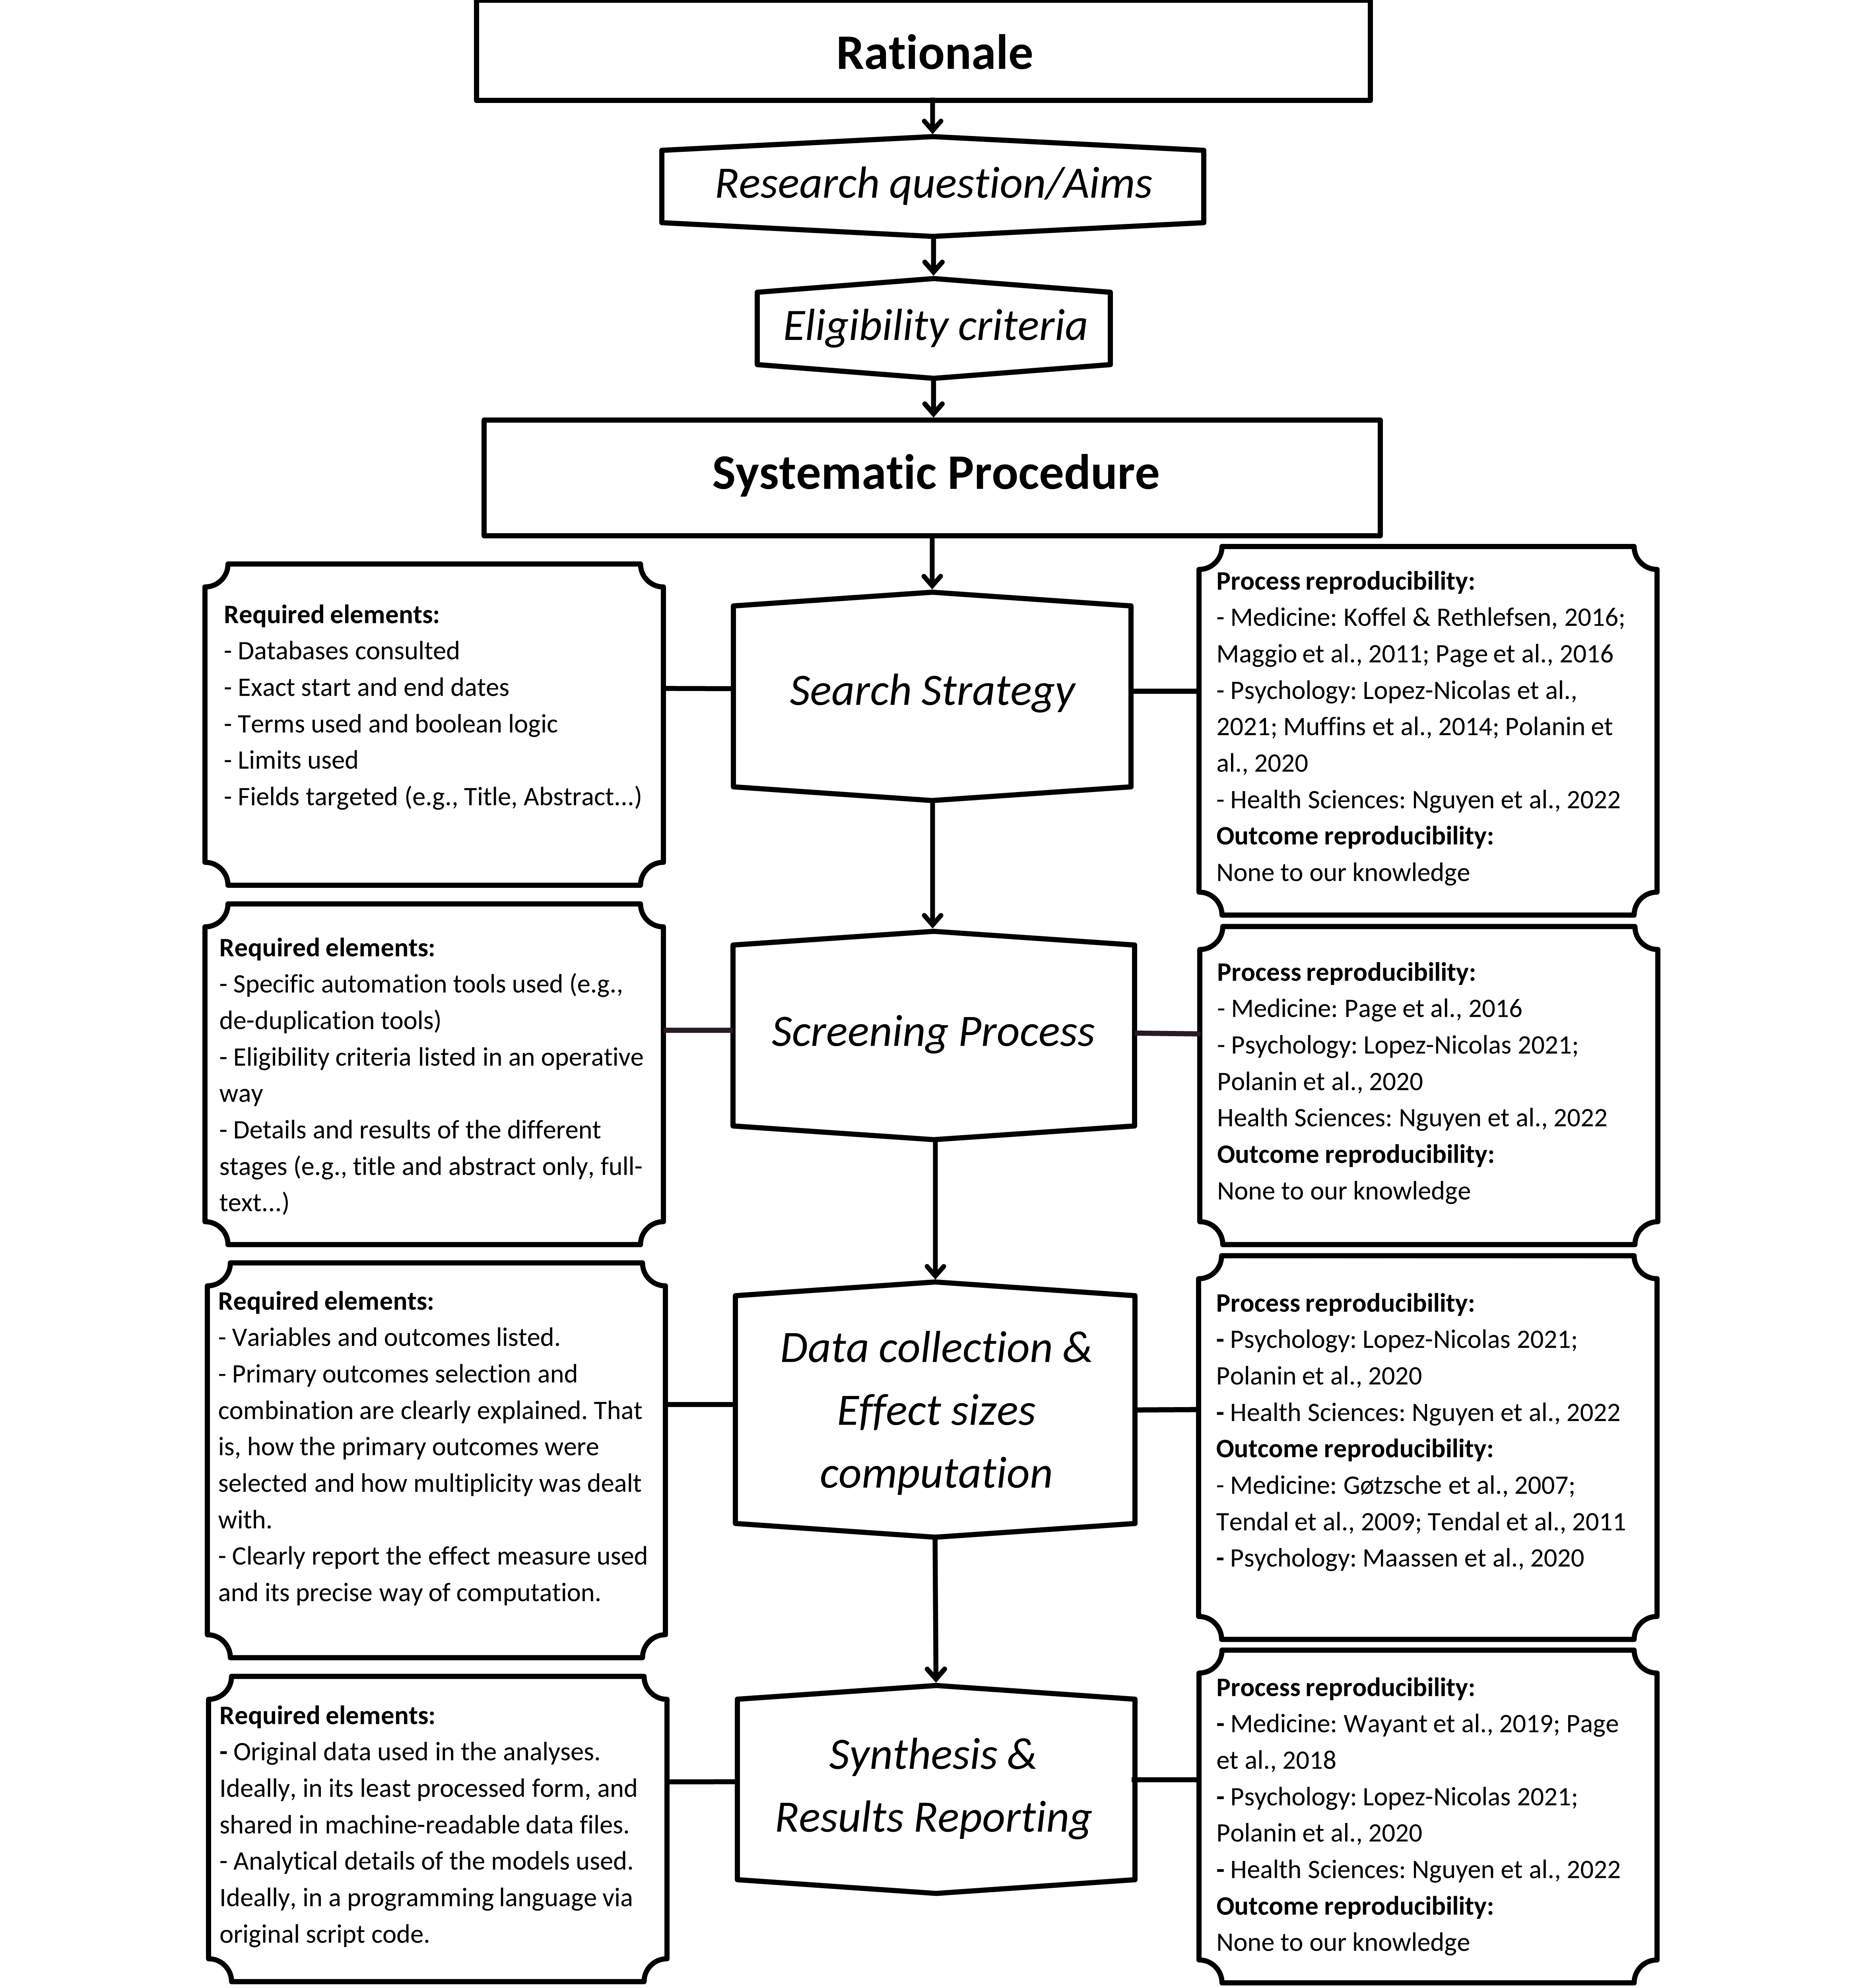
\includegraphics[width=\textwidth, height=\textheight]{results/Figure 1.png}

\caption{Flowchart displaying the basic pipeline of a meta-analysis. Each of the stages may be subject to reproducibility evaluation. On the left, known studies that have evaluated some facet of the reproducibility of each stage are listed. On the right, the various elements that must be available to reproduce each stage are enumerated.
}

\label{fig:figs1}
\end{center}
\end{figure*}

Reproducibility analysis typically uses the original data available from the original authors (e.g., Artner et al., 2020; Hardwicke et al., 2021, 2018). This puts the focus of the assessment at factors such as the reusability of the available data, challenges for the reconstruction of the original analysis scheme, reporting errors, etc. Although data availability seems to have improved in the last years (Hardwicke et al., 2018; Tedersoo et al., 2021; Wallach et al., 2018), systematic reviews and meta-analyses appear to be a special case. Typically, the data collected for a meta-analysis is study-level summary data extracted from published primary studies which is commonly reported in the paper through tables or forest plots. This may lead to the idea that common data sharing practices do not apply to meta-analysis. For example, Page et al. (2022) analysed the content of data availability statements from a set of meta-analyses published in 2020. Only 31\% included a data availability statement and only 13\% of these included a link to access the data openly, with 23\% stating that all relevant data are available in the paper itself, 10\% stating that data sharing is not applicable as no datasets were generated, 8\% stating that data sharing is not applicable as the data is drawn from already published literature, and 42\% stating that data were available upon request. It is surprising that, even just considering meta-analyses that included a data availability statement, the authors of these meta-analysis assume that such practices do not apply to meta-analyses or that the data in the article itself is sufficient.

\hypertarget{purpose}{%
\subsection{Purpose}\label{purpose}}

Previous research has revealed that there is room for improvement at different stages of the meta-analytic process pipeline. In this study our purpose is twofold. First, we broadened previous process reproducibility assessments by considering data availability on request and by contacting original authors to request required information to reproduce the meta-analysis. Second, we verified the outcome reproducibility of the meta-analyses that were process-reproducible using the available data. Where previous work focussed on the reproducibility of primary effect sizes, we explored meta-analysis outcome reproducibility using the primary effects sizes already coded by the original authors.

\hypertarget{method}{%
\section{Method}\label{method}}

\hypertarget{preregistration}{%
\subsection{Preregistration}\label{preregistration}}

The pre-data analysis protocol (\url{https://doi.org/10.17605/OSF.IO/79J2T}) was pre-registered on 19 October 2021. Any deviation from this protocol is explicitly acknowledged.

\hypertarget{data-materials-and-online-resources}{%
\subsection{Data, materials, and online resources}\label{data-materials-and-online-resources}}

Data and analysis script code are openly available at: \url{https://osf.io/6cmzh/}

\hypertarget{identification-and-selection-of-articles-and-meta-analyses}{%
\subsection{Identification and selection of articles and meta-analyses}\label{identification-and-selection-of-articles-and-meta-analyses}}

In previous research we identified a pool of 664 meta-analytic reports on clinical psychological interventions published between 2000 and 2020 through a systematic electronic search (López-Nicolás et al., 2022). Of this pool, 100 were randomly selected using a random number generator between 1 and the total number of meta-analyses identified. The full search strategies and a summary of the screening process are available at: \url{https://osf.io/z5vrn/}, and the workflow of the random selection process is available at: \url{https://osf.io/cp293/}.
From these 100 articles, each independent reported meta-analysis with at least 10 primary studies was selected. In case no meta-analysis reported in a paper had at least 10 studies, the meta-analysis with the highest number of primary studies was selected, which was the case for 29 of the articles included in this report. Our unit of analysis was each independent meta-analysis selected under these criteria. A total of 217 independent meta-analyses were selected.

\hypertarget{retrieval-of-primary-data}{%
\subsection{Retrieval of primary data}\label{retrieval-of-primary-data}}

The availability of necessary primary data was checked. First, we searched for machine-readable data files through links leading to third-party repositories or in supplementary material hosted by the journal. Second, we looked for available data through tables or forest plots in the meta-analytic report itself, or in supplementary material. In these cases, the primary data had to be manually re-coded to reuse it. Finally, if the primary data of a meta-analysis were not directly available after the previous steps, we attempted to obtain the data through a request to the corresponding author identified in the associated paper. We sent an initial request in June 2021 and, if there was no reply, a subsequent reminder in October 2021. This reminder was sent to a more recent alternative email address if we were able to find one. If we were unable to obtain the data through the email request, the associated meta-analysis was labelled as not process reproducible.

In order to be able to reproduce meta-analyses, primary effects and their associated standard errors are required. These are generally computed from primary statistics retrieved from the primary studies such as means, standard deviations or sample sizes. We attempted to retrieve the least processed data possible. First, we sought for the primary statistics, recovered in 26\% of the cases. Second, we sought for the primary effects and their standard errors (or, alternatively, the sampling variances), recovered in 5\% of the cases. Finally, we sought for the primary effects and their confidential limits, recovered in 69\% of the cases, from which the standard errors were approximated as follows:

\[se_i = (\frac{UB_i - LB_i}{2z_{\alpha/2}})\]

with \(se_i\) being the standard error of the ith effect size, \(UB_i\) and \(LB_i\) the upper and lower confidence limits of confidence interval for the ith effect size, and \(z_{\alpha/2}\) the \(1 - z_{\alpha/2}\) quantile of the standard normal distribution (usually, \(z_{\alpha/2} = 1.96\) assuming a two-sided 95\% confidence interval).

\hypertarget{reconstructing-the-original-analytical-scheme}{%
\subsection{Reconstructing the original analytical scheme}\label{reconstructing-the-original-analytical-scheme}}

To proceed with reproducibility attempts of the meta-analyses that were labelled as process reproducible, we first looked for the availability of the original analysis script. When it was available, analytical reproducibility was checked by rerunning the original script on the associated primary data. In 141 cases (97\%), the analysis script code was not available. In these cases we tried to reconstruct the original analytical scheme using the technical details reported in the paper. Specifically, we collected information on: (a) the meta-analytic model originally assumed; (b) the weighting scheme; (c) the between-studies variance estimator; (d) the method used to compute the confidence interval; and (e) the software used to perform the meta-analysis. If any of these details about the analytical methods were not reported, but the software used was mentioned, we inferred the first four pieces of information from the default settings of the software used. If the software used was not reported, we inferred this information from the default settings of the most used software in the sample, which was \emph{Comprehensive Meta-Analysis}.

Additional information about the meta-analysis was collected that is not reported in this manuscript. The full list of variables collected is available in the Protocol (\url{https://osf.io/tq4uf/}) and a Codebook describing these variables is available at: \url{https://osf.io/ym78s/}.

\hypertarget{data-collection-procedure}{%
\subsection{Data collection procedure}\label{data-collection-procedure}}

Primary-level data and aggregate-level data described above were coded by five members of the group. At a first pilot stage, a random sample of five articles of the total pool was independently coded by the five members and, subsequently, in a series of meetings, disagreements between the coders were resolved by consensus. Next, the initial pool of 100 included articles was split among four coders, 25 articles each. A random sample of 25 articles of the total pool was assigned to the fifth member to carry out independent double-coding, with the goal to examine the reliability of the data collection process. Disagreements were resolved by consensus and by double-checking the original materials.

\hypertarget{reproducibility-outcomes}{%
\subsection{Reproducibility outcomes}\label{reproducibility-outcomes}}

Each meta-analysis was labelled using the following reproducibility success scheme: (a) reproducible; (b) not process-reproducible; (c) numerical error, and (d) decision error. Not process-reproducible refers to situations where we were unable to access the primary data neither through direct extraction nor upon request. Similar to previous studies (Artner et al., 2020; Hardwicke et al., 2018, 2021) an index of numerical error was computed (see Protocol \url{https://osf.io/tq4uf/}). This index expressed the difference between reproduced and original values as a percentage. To avoid labelling minor numerical discrepancies related to numerical rounding as reproducibility problems, a 5\% discrepancy threshold was set. Thus, a meta-analysis was labelled as `numerical error' if it showed a discrepancy larger than 5\%.\footnote{A sensitivity analysis using other possible criteria is reported in the supplementary file.}
Finally, the label `decision error' refers to situations where the \(p_{reported}\) fell on the opposite side of the .05 boundary in relation to the \(p_{reproduced}\).

We focus on analytical reproducibility of summary effects, their confidence bounds and the result of the null hypothesis significance test. Secondarily, we also assessed analytical reproducibility of other synthesis methods such as heterogeneity statistics.

\hypertarget{reproducibility-checks-workflow}{%
\subsection{Reproducibility checks workflow}\label{reproducibility-checks-workflow}}

Analytical reproducibility checks were carried out at different stages. First, through reported analytic details or script code. When the analysis script code was available, computational reproducibility was checked by rerunning the script with the available primary data. In most cases, the analysis script code was not available. Thus, in these cases we coded the analytic details as explained above to fit equivalent meta-analytic models as a function of these details using the available primary data. This analysis scheme was programmed in the R environment (R Core Team, 2022) using the \emph{metafor} package (Viechtbauer, 2010).

Second, given that the manual recoding process is an error-prone task, some mistakes can appear. Thus, those meta-analyses labelled as numerical error and/or decision error in the previous stage were re-assessed by a different member of the team. In cases where an error was found in the originally coded results, analytic methods and/or primary data, the meta-analyses were once reproduced again and re-labelled according to the updated results. Additionally, a qualitative assessment of the meta-analyses still labelled as numerical error and/or decision error was also carried out. The same reviewers who checked for errors produced individual reports on the possible source of the discrepancy and its reproducibility was judged qualitatively by four of the other authors. This stage was a deviation from the pre-registered protocol, and made it possible to identify situations with obvious explanations, such as rounding issues, inverted signs, etc.

Finally, for meta-analyses that remained labelled as non-reproducible, an email was sent to the corresponding author of the associated paper explaining our aims, our approach, and our results regarding his/her meta-analysis and requesting additional information that could explain the mismatch between the original reported results and the reproduced results. We tried to solve the reproducibility issues within a month after the request and we updated the label accordingly.

\hypertarget{results}{%
\section{Results}\label{results}}

From the 100 included papers, 217 independent meta-analyses were selected following the criteria explained above. These meta-analyses included 18.35 primary studies on average (sd = 17.25; median = 13; interquartile range = 10-19; range = 3-134)). Figure 2 displays the distribution of number of primary studies among the meta-analyses included in our sample. Original results and characteristics of these meta-analyses are available at: \url{https://osf.io/8jzbk}

\begin{figure}
\centering
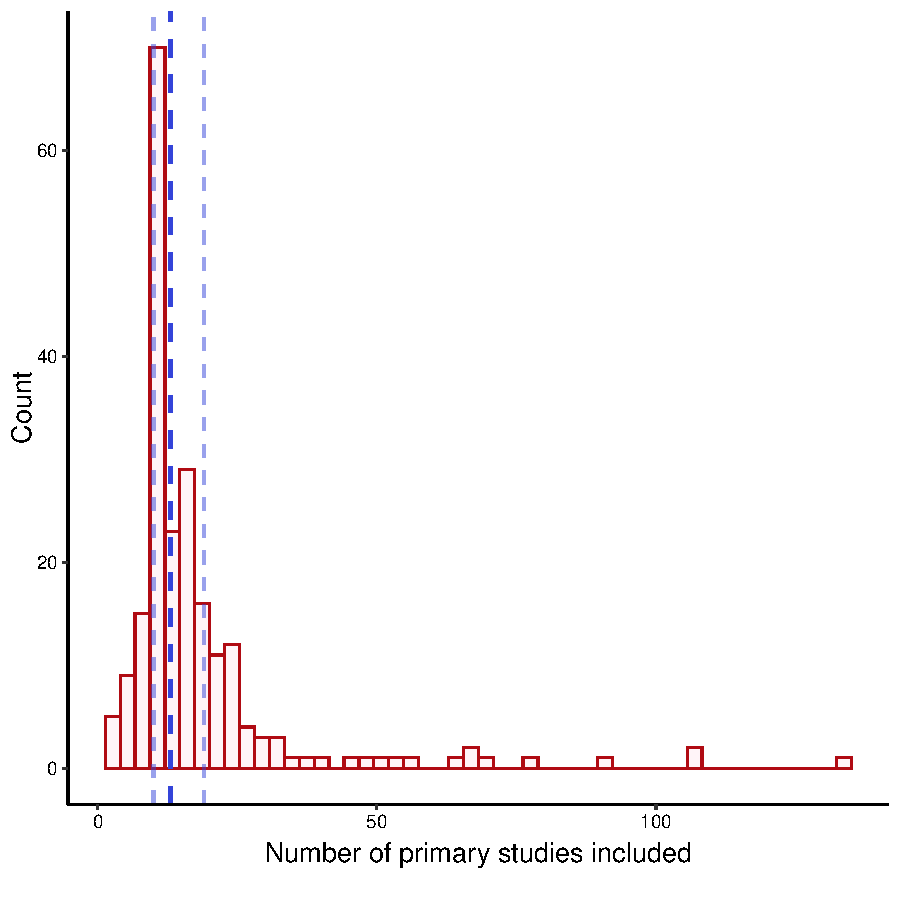
\includegraphics{manuscript_files/figure-latex/unnamed-chunk-1-1.pdf}
\caption{\label{fig:unnamed-chunk-1}Distribution of the number of primary studies included in each of the meta-analyses. Vertical blue dotted lines represent the first quartile, median, and third quartile, respectively.}
\end{figure}

\hypertarget{process-reproducibility}{%
\subsection{Process reproducibility}\label{process-reproducibility}}

Figure 3 summarizes the primary data retrieval results. Based on the availability of primary data, either retrieved directly from the paper or upon request, 146 meta-analyses (67\%, see Fig. 2a) were labelled as process reproducible. Of these 146 meta-analyses, in about half of the cases the primary data was retrieved from a forest plot in the paper itself and in about a third of the cases the primary data was retrieved from supplementary files. Only in 3\% of the cases the primary data was retrieved upon request (see Fig. 2b for further details). Although attempts were made to retrieve data for 75 meta-analyses from 25 different papers by emailing the corresponding authors, data was only retrieved for 4 meta-analyses, from 3 different papers (12\%, see Fig. 2c). For the remaining 71 from 22 different papers, a reply providing some reasons not to share was received in 12\% (see Fig 2c), whereas no reply was received for the remainder of the meta-analyses. Table 1 summarises the different reasons corresponding authors given when data was not provided upon request.

\begin{table}

\caption{\label{tab:unnamed-chunk-2}Reasons given when data was not received upon request.}
\centering
\begin{tabular}[t]{>{\raggedright\arraybackslash}p{7cm}cc}
\toprule
Reason & N & \%\\
\midrule
Data held by a co-author, and do not have his contact details & 1 & 12\%\\
Propietary dataset & 1 & 12\%\\
The author no longer has the data. & 5 & 62\%\\
The author requested more information and a written agreement including possible authorship. 
                                                      Additional details were sent and after some email exchanges there was no further response. & 1 & 12\%\\
\bottomrule
\end{tabular}
\end{table}

\hypertarget{challenges-faced-retrieving-primary-data}{%
\subsection{Challenges faced retrieving primary data}\label{challenges-faced-retrieving-primary-data}}

In most cases, when the meta-analytic data was available, it was shared in document formats, as previously reported. Data available in tables or forest plots shared in \emph{pdf} or \emph{docx} format --either in the document itself or in the supplementary materials-- was found to be highly prevalent. This required a manual recoding of the primary data to be able to reuse them. Furthermore, when data was reported through general tables (i.e.~tables listing all the primary studies included with their characteristics), the meta-analysis associated with each data entry was not always obvious, leading to the time-consuming task of matching each data entry with each independent meta-analytic result reported in the paper. There were only 7 meta-analyses (from three different papers) of the 146 meta-analyses labelled as process reproducible (5\%), where the task of retrieving the data required simply downloading the data in an machine-readable data file format.
On the other hand, as shown in Figure 3c, when the necessary data was not available, retrieving it upon request to the original authors led to a remarkably low reponse rate.

\begin{figure*}
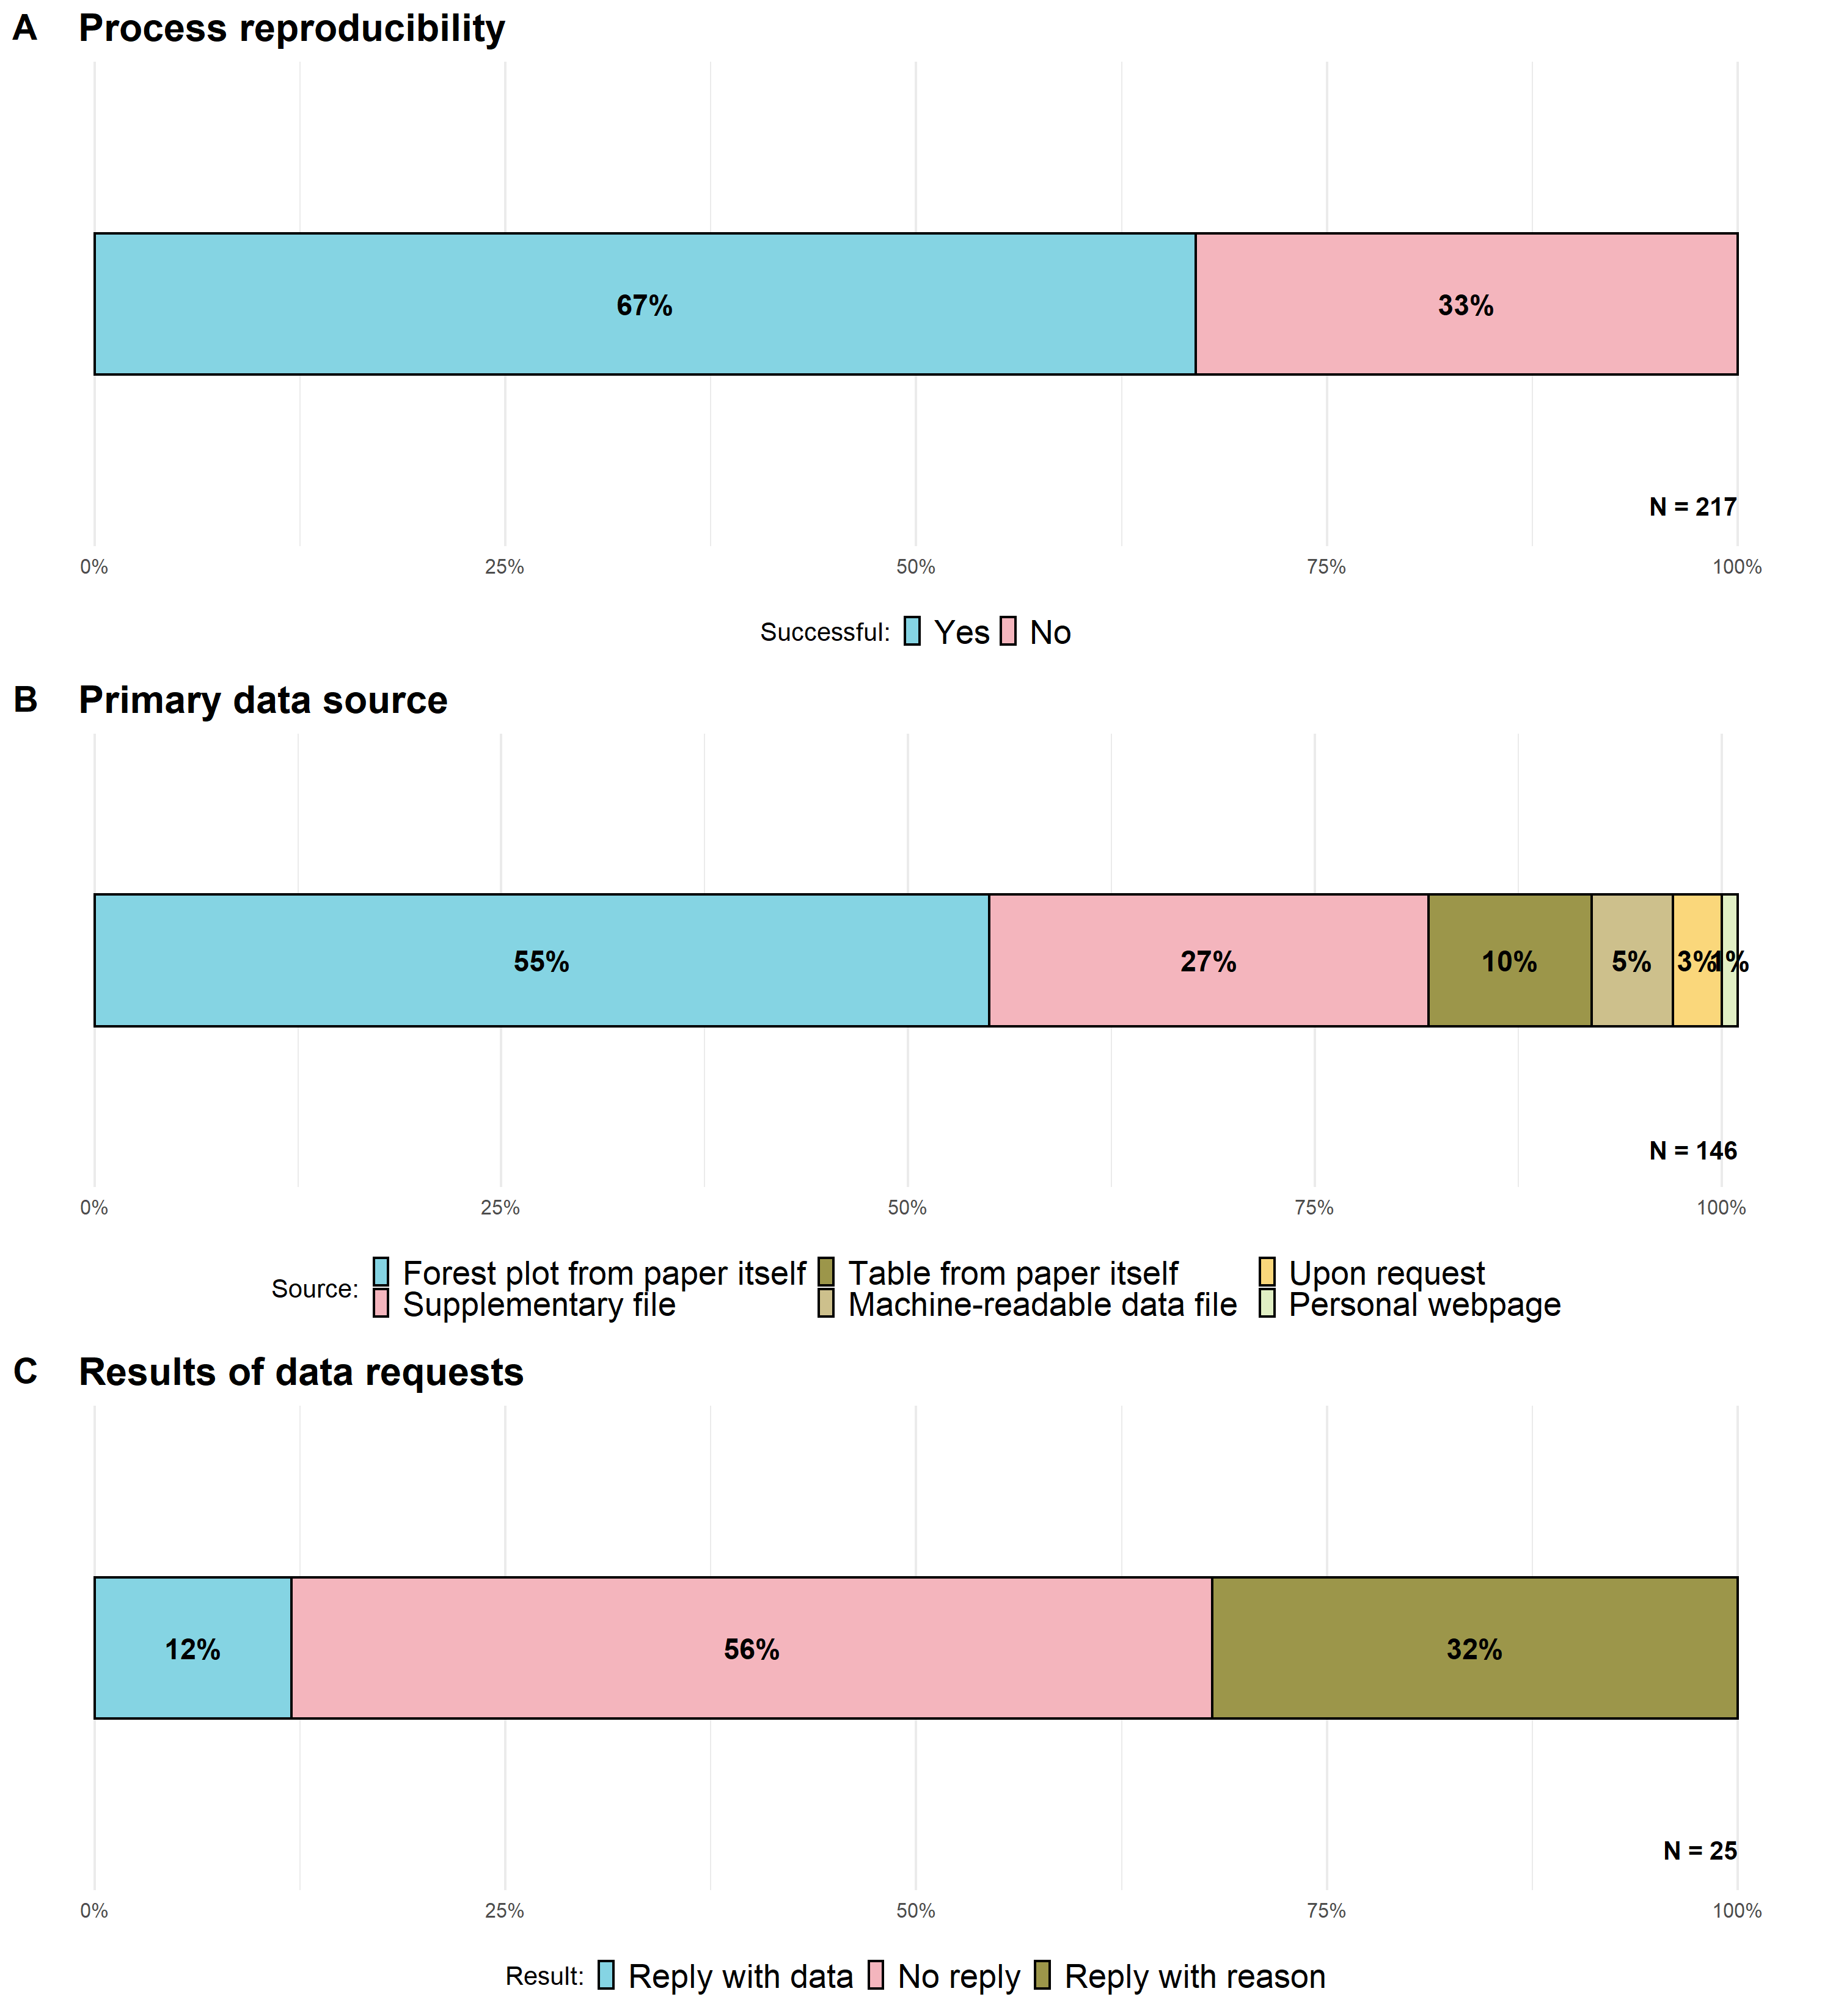
\includegraphics[width=1\linewidth]{manuscript_files/figure-latex/unnamed-chunk-3-1} \caption{Percentage of (a) process-reproducible meta-analyses; (b) different types of sources of original data; and (c) data request results.}\label{fig:unnamed-chunk-3}
\end{figure*}

\hypertarget{outcome-reproducibility}{%
\subsection{Outcome reproducibility}\label{outcome-reproducibility}}

The outcome reproducibility was checked in 146 meta-analyses from 82 different papers. As mentioned above, in 5 of these meta-analyses (3\%), all from the same published article, the original script code was available. Therefore, in these five cases, analytical reproducibility was checked running the original analysis script on the original primary data. In the remaining cases, the original analytical framework was reconstructed as explained in the method section.

Following the first stage of re-analysis, 52 meta-analyses were re-assessed because they were labelled as numerical error and/or decision error.

Of these, 17 were re-analysed again as some coding errors were found in the second stage. After this, 10 were re-labelled as reproduced and 7 still had relevant discrepancies. Furthermore, 15 were labelled as reproduced in the qualitative check because the discrepancy was probably explained by rounding issues, inverted signs for results (where effect sizes were reported in absolute values) and primary data, minor reporting errors, or minor adjustments in the analytical scheme. In the remaining 20, and in the 7 re-analysed again without success, some issues or relevant discrepancies without apparent explanation were found.

Figure 4 displays a scatterplot showing the consistency between the original and reproduced summary effect size and their confidence bounds of these 52 meta-analyses.
Additionally, as a secondary analysis, the reproducibility of the \(I^2\) heterogeneity statistic was explored. Figure 5 displays a scatterplot showing the consistency between the original and reproduced \(I^2\) statistics. As shown in Figures 4 and 5, the discrepancies found in the heterogeneity statistic \(I^2\) are larger than those found in the summary effects and their confidence intervals. The lack of precision of the available data (rounded data) or incomplete information on aspects such as the tau-squared estimator applied seem to have a substantial impact on the reproducibility of this result.

\begin{figure}
\centering
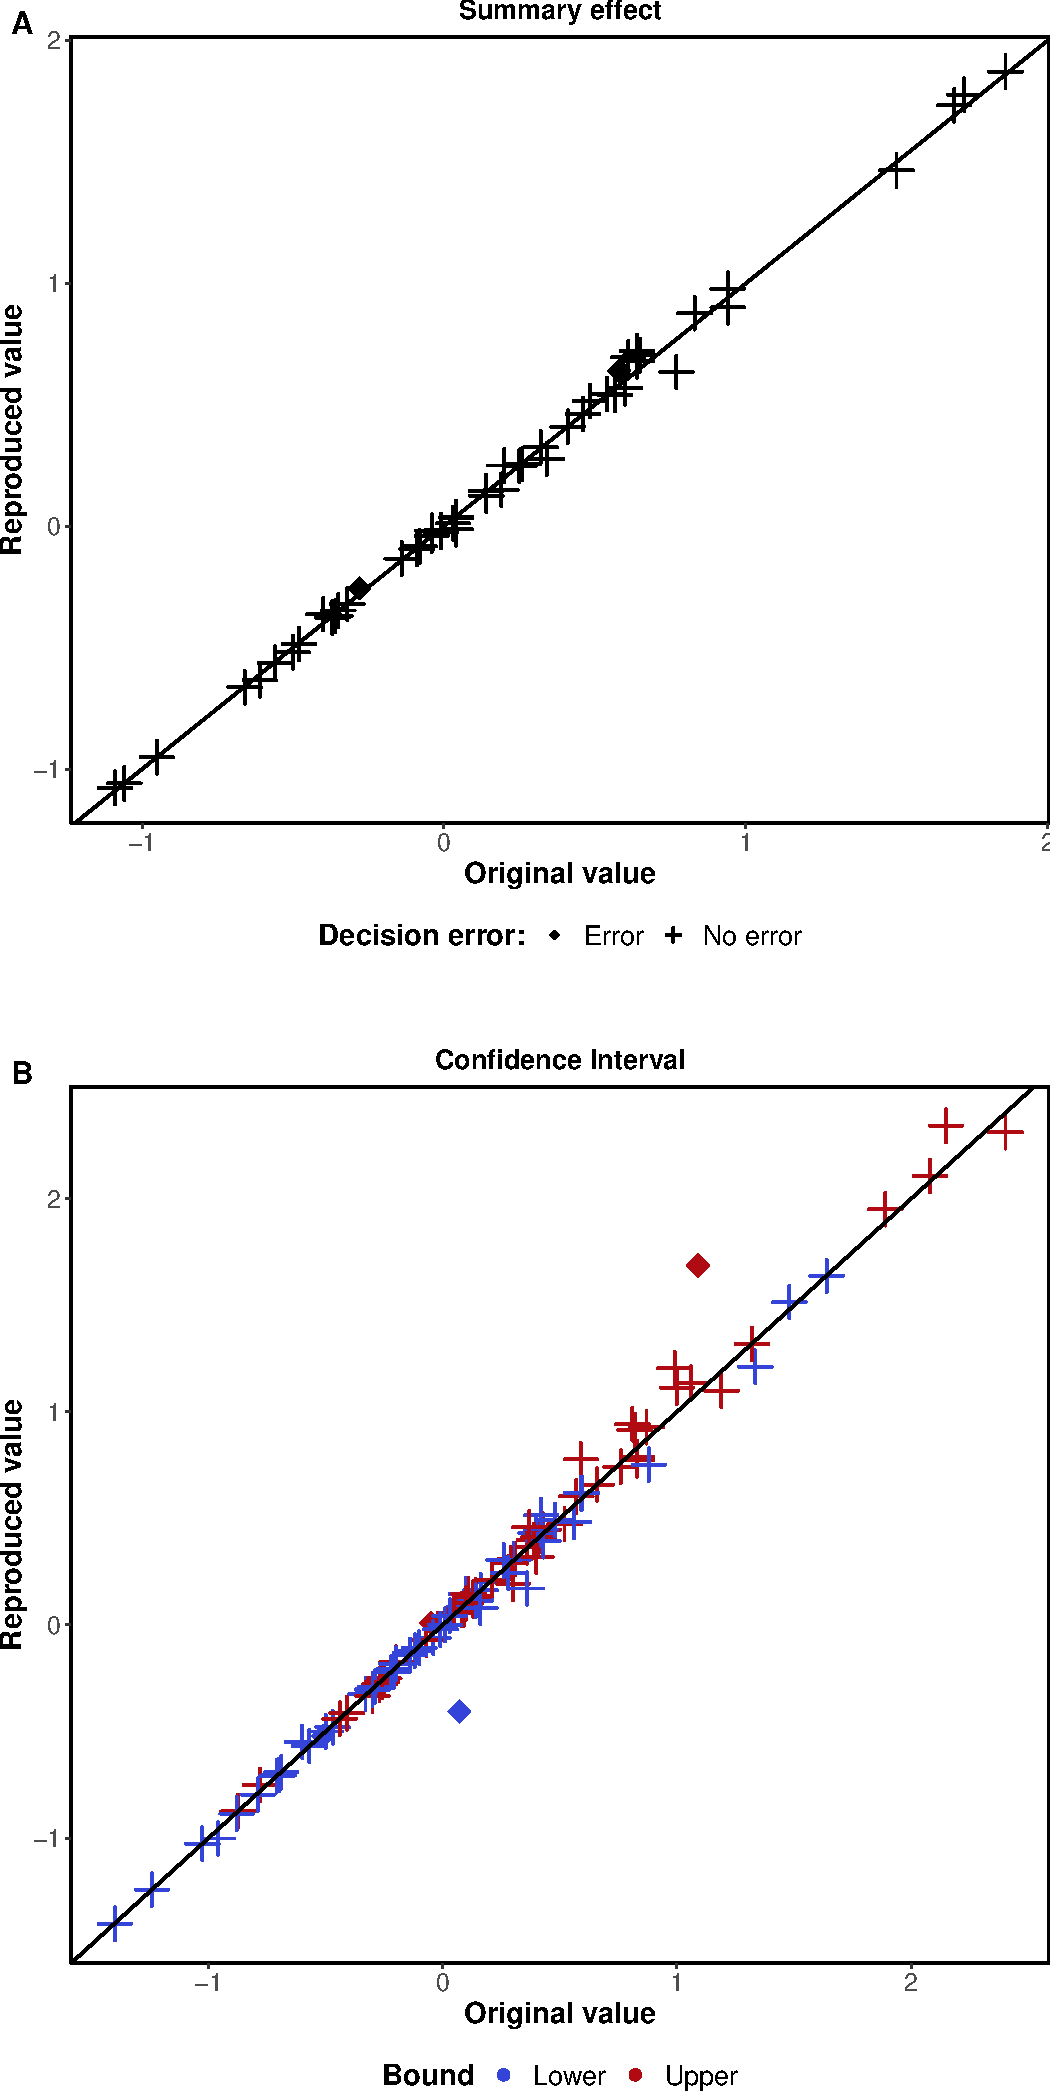
\includegraphics{manuscript_files/figure-latex/unnamed-chunk-4-1.pdf}
\caption{\label{fig:unnamed-chunk-4}Scatterplot displaying the reproduced values as a function of the original values classified by whether or not decision error was found. Only the results of the 52 meta-analyses with a discrepancy of more than 5\% identified in the first stage are displayed, but with the corrections made in the second stage. In panel (a) the summary effects are displayed and in panel (b) the confidence intervals. For (b) the colours represent lower or upper bound of the confidence interval.}
\end{figure}

\begin{figure}
\centering
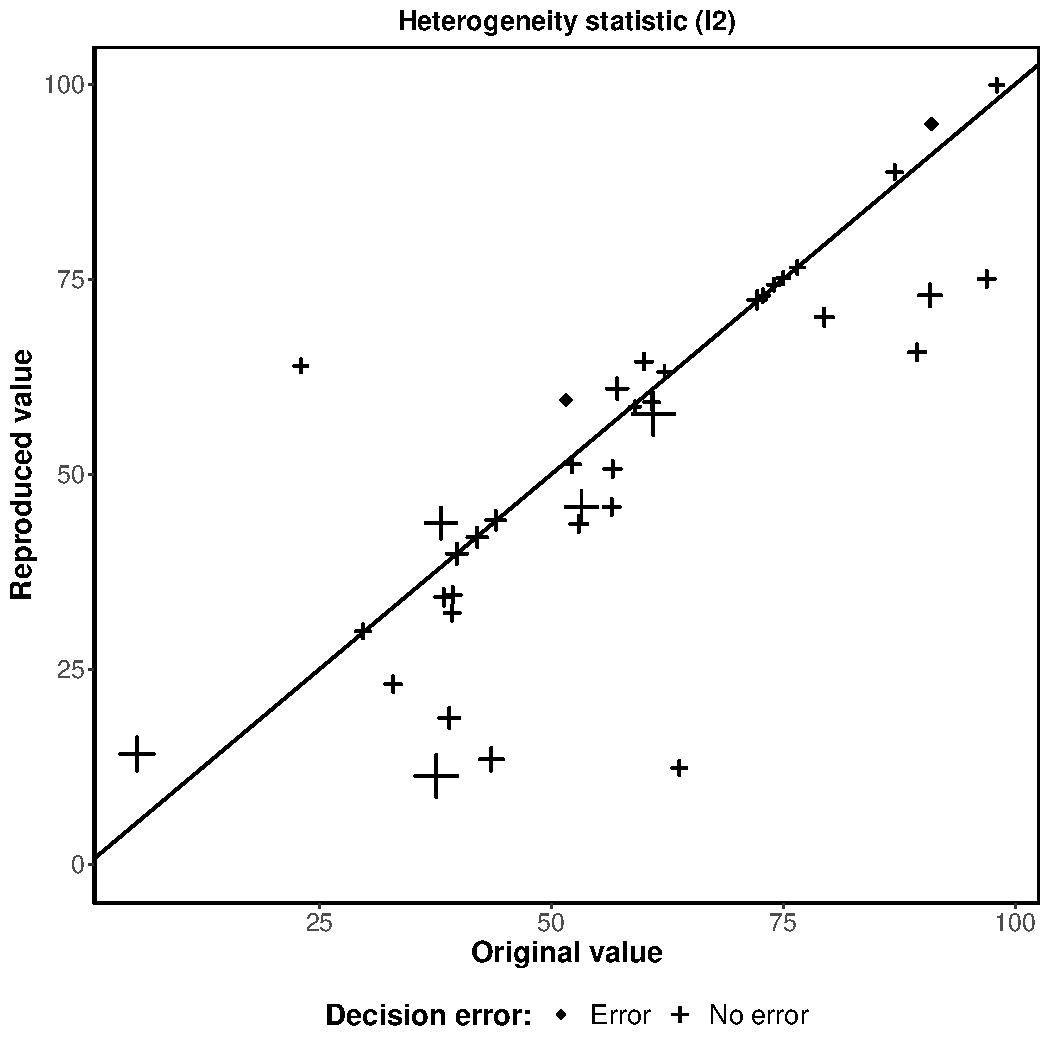
\includegraphics{manuscript_files/figure-latex/unnamed-chunk-5-1.pdf}
\caption{\label{fig:unnamed-chunk-5}Scatterplot displaying the reproduced values as a function of the original values classified by whether or not decision error was found. Only the results of the 52 meta-analyses with a discrepancy of more than 5\% identified in the first stage are displayed, but with the corrections made in the second stage. The values displayed are \(I^2\) hetorogeneity statistics. The size of the crosses is function of the discrepancy in the summary effect.}
\end{figure}

\hypertarget{main-issues-identified}{%
\subsection{Main issues identified}\label{main-issues-identified}}

Different issues in these 27 meta-analyses were identified in the second stage. For example, for one of the meta-analyses which showed a discrepancy in the confidence limits, inconsistencies were found in the original meta-analytic report itself. The confidence limits originally reported for that meta-analysis were different in the abstract, main text and forest plot. Matching the reproduced results were those reported in the forest plot but not those reported in the text. Furthermore, inconsistencies in the original summary effect reported were found between the results reported in abstract and the results reported in the main text and the forest plot. This example of inconsistencies in original results was also found in other cases. Also, in a paper where primary data were available in both a table and a forest plot, minor inconsistencies were found between the primary data of the table and the forest plot. These appeared to be typos.
Furthermore, some inconsistencies were found with respect to the number of primary studies included in each meta-analysis. For example, in one of the meta-analyses, the main text reported the inclusion of 10 comparisons in the meta-analysis, whereas in a table of results 11 comparisons were reported for this meta-analysis. On the other hand, in 11 meta-analyses the primary data retrieved from the supplementary materials were not sufficient to reach the number of primary studies stated as included in this meta-analysis in the original report.

\hypertarget{original-authors-clarifications}{%
\subsection{Original authors clarifications}\label{original-authors-clarifications}}

These 27 meta-analyses were from 10 different papers. Therefore, 10 clarification requests with information about the study aims, methods and preliminary results were sent to the corresponding authors of the original articles. A reply was received in only 2 of the 10 cases.
In one of them, the original authors sent back a link to an OSF repository where the original data and analysis script were stored. According to the authors, this link was not reported in the paper by mistake. The script was run on these data and the results were successfully reproduced. In this case, the data previously used were retrieved from a forest plot (means and standard deviations) and a table (sample sizes) reported in the paper. The previous discrepancy was explained by two cases included in the original meta-analysis from the same primary study that were reported with the same ID in the forest plot and were not correctly matched with their corresponding sample size extracted from the table. This situation exemplifies the potential issues arising from having to reconstruct the original data from tables and figures and not having open access to the original data file.

In the other case, the original data was retrieved from a huge table in supplementary material with all effect sizes and their confidence limits. The original authors sent back this same table by increasing the number of decimal places of the effect sizes and after correcting some wrong values that they themselves detected in that process. This fixed the discrepancies for some of the meta-analyses in this paper.

Figure 6 summarises the results of the whole process of outcome reproducibility assessment.

\begin{figure*}
\begin{center}
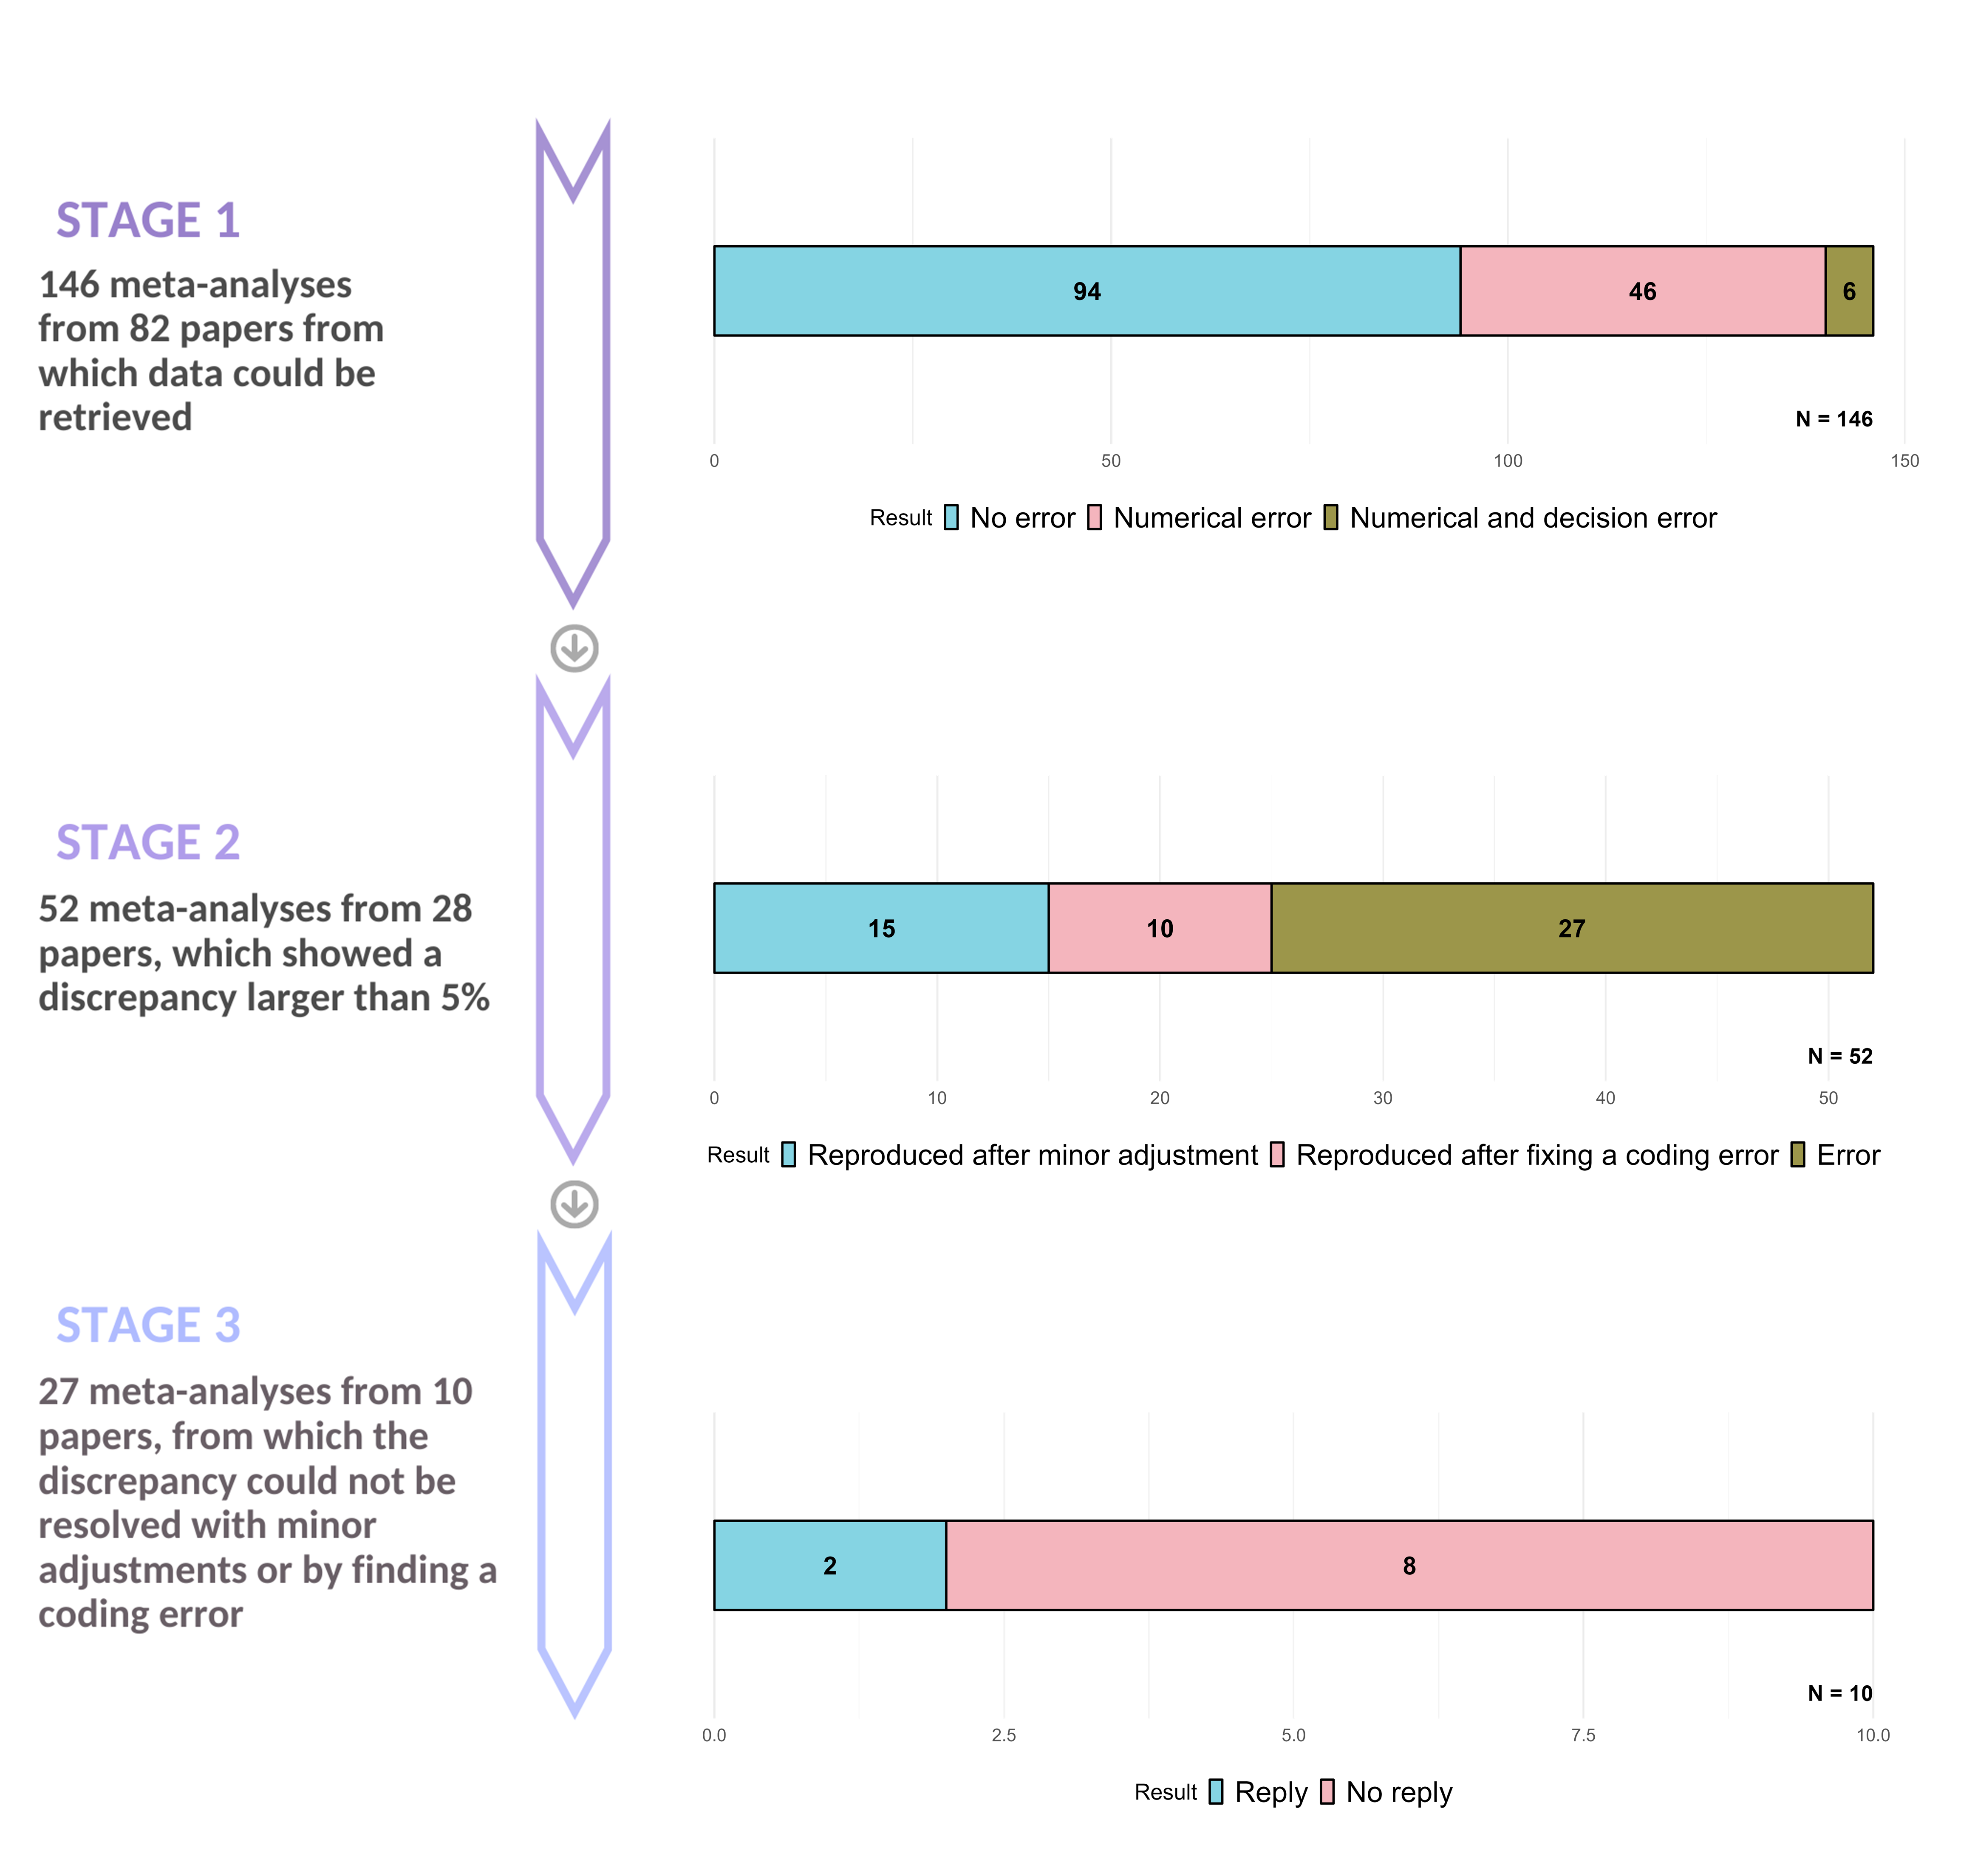
\includegraphics[width=\textwidth]{results/Figure 6.png}

\caption{Results of the different stages carried out in the evaluation of the outcome reproducibility. 
}

\label{fig:fig6}
\end{center}
\end{figure*}

\hypertarget{discussion}{%
\section{Discussion}\label{discussion}}

The main aim of this study was to examine the analytical reproducibility of a sample of published meta-analyses on the effectiveness of clinical psychology interventions. We analyzed the availability and reusability of original data and, assessed the reproducibility of the published results using these retrieved original data, and tried to reconstruct the original analysis plan. We encountered both difficulties in retrieving the original data and some problems with the reproducibility of the meta-analyses examined.

Even when we interpret data availability in the broad sense (i.e.~retrieving data from tables and figures when no data file was available), for about a third of the included meta-analyses no data was available. In these cases, attempts were made to obtain the data on request to the corresponding author, with little success. Authors only shared data in 12\% of the requests that were made. This result is in line with what was found in a recent study where data availability statements from a set of primary studies were analysed (Gabelica et al., 2022).Where 42\% of primary studies in Gabelica et al. (2022) reported data was available on request (and identical percentage was found in Page et al. (2022) for meta-analyses), only 6.8\% of the authors shared the underlying data when requested. Even though it is common to see authors state data is available on request, actually obtaining the data on request seems highly challenging. Although this problem of retrieving data on request is well known (Wicherts et al., 2006), the situation does not seem to have improved. Nowadays, there are straightforward, free, and open ways to share data, including meta-analytic data files. Several repositories (e.g., OSF, GitHub, Zenodo, Figshare) are available for researchers to openly share the data associated with published results. On-request availability has proven to be inadequate, and with the availability of data repositories is no longer necessary. Journals publishing meta-analyses should require that authors share the underlying data in a public data repository.

For the remaining meta-analyses (about two thirds), we were able to retrieve the data used by the original authors. In only 5\% of these cases data was shared in a machine-readable data file (e.g., \emph{csv}, \emph{xlsx}), while the data had to be retrieved from files in document format (e.g., \emph{docx}, \emph{pdf}) for the rest of cases. This forces people who want to re-use the data to manually recode the data, which is both inefficient and error-prone task. Even after partial double coding was carried out, this procedure did not avoid some coding errors, which were detected by double checking meta-analyses with discrepancies. In out experience, the data retrieval process can be difficult when results are presented in general tables, as it involves matching subsets of these primary data with different meta-analytic results, while is not always clear which studies were used in which meta-analysis reported in a paper. Furthermore, because the tables in manuscript are often generated manually in document file formats (e.g.~Word), we observed examples where this introduced another source of error. There are good guidelines on how to share research data properly (Wilkinson et al., 2016), and authors should share data in machine-readable formats.

An important finding is that the availability of the original analysis script was very limited. Only in five meta-analyses (3\%, all from the same paper), was the original script openly available. In most cases, the original analyses were reconstructed from the description provided in the paper itself, which was not always rich in detail, so that many of these computational details had to be inferred from the default settings of the software authors used. The availability of analysis scripts often shows similar rates, both in meta-analyses (Page et al., 2022; Polanin et al., 2020) and in primary research (Hardwicke et al., 2022, 2020). This makes it more difficult to easily check the computational reproducibility of the results from such studies. Reconstructing the analytical scheme adds to the workload, with the potential to introduce errors, both in the original report and in the reconstruction, and deals with the eventual lack of relevant analytical information. With the increasing availability of excellent open-source tools to perform meta-analysis (e.g., \emph{metafor} (Viechtbauer, 2010) in R) and useful templates (Moreau \& Gamble, 2020), meta-analysts can use workflows that allow them to create and share analysis code for meta-analyses.

Despite these difficulties, we were able to recover the original data and reconstruct the original analysis approach, for 146 meta-analyses, for which the analytical reproducibility of the results was assessed. These attempts at analytical reproduction went through several stages as explained above, trying to minimize the impact of possible coding errors, and requesting clarifications from the original authors. Nevertheless, even with these efforts, some discrepancies remained in the results. We identified different issued that hindered our reproducibility attempts. For example, in some cases internal discrepancies were found in the paper itself (e.g., text-figure discrepancies, text-abstract, or text-table discrepancies). Furthermore, some problems were found with the lack of some primary data, where data available in the supplementary material included fewer cases than those finally reported in the results of the published paper. These situations could be explained by typos in the manuscript, or updates when performing the meta-analysis that produced different versions of the manuscript, data, or supplementary material. While it is important to note that discrepancies in the summary effect results and their confidence intervals were mostly minor, with little or no impact on the conclusions, these situations are easily avoidable. Some of the problems identified could be explained by typos. Currently, there are tools that facilitate the production of so-called reproducible manuscripts, such as the R packages \emph{kintr} (Xie, 2022), \emph{rmarkdown} (Allaire et al., 2022), and \emph{papaja} (Aust \& Barth, 2022). A reproducible manuscript embeds analysis code, data and results reporting in a single document, extracting and reporting the results from the output of the computational process itself, avoiding error-prone manual transcriptions.

Our results are complementary to those observed in previous research on the reproducibility of the primary effects of meta-analyses (Gøtzsche et al., 2007; Maassen et al., 2020) and related problems due to the multiplicity of primary effects (Tendal et al., 2009). These studies found problems in reproducing the primary effects of published meta-analyses, or in reaching agreement between independent coders in computing them. Such problems, to a greater or lesser extent, had some impact on the meta-analytic results. Our results show that, even when re-using the primary effects as originally coded, certain problems of reproducibility of the results may remain. Some of these problems are added error on the source of error found in previous research on reproducibility of primary effects, which in turn are added error on the sources of error types of primary estimates (e.g., measurement error, sampling error, or reporting errors). No scientific research is totally error-free, but one of the main tasks of scientists is to minimize this error, and in some cases, such as those observed in this study, minimizing some potential sources of error can be straightforward.

Our study has some limitations. First, the time span covered is fairly wide. Thus, the findings may not capture the changes that have arisen in recent years. Therefore, future studies should examine more specific changes over years, to evaluate whether better practices emerge that facilitate reproducibility. Second, most of the primary data was retrieved through manual re-coding, which introduces some error. The reported data was rounded, which means we did not have access to precise values, and in many cases the standard error had to be approximated from the confidence limits. These limitation of our study are caused by the suboptimal practices when sharing data we discussed above. Given the non-precise nature of most of the data retrieved, we had to make a decision about which margin of discrepancy was acceptable. In this study, a margin of 5\% was chosen. Because this cut-off is arbitrary, we have tried to focus more on possible issues in the results that fell above this margin, than on establishing a exact ratio of non-reproduced meta-analyses based on this arbitrary cut-off.

In conclusion, we observed several difficulties when attempting to reproduce meta-analyses. Two aspects can be highlighted: (1) data availability and reusability of the data as they are shared, (2) and apparent errors in the reporting of results. As data collected for a meta-analysis can be especially useful for future research, direct and open access to such datasets allows for easy updates, and re-analyses, which are valuable in a cumulative science. Meta-analytic data generally do not contain sensitive or personal information, and can therefore almost always be shared openly, as doing so does not involve ethical or legal conflicts. Third, meta-analytic results often represent the state of the art of the evidence on a particular topic. These results guide applied practice, public policy, or future research directions. This prominent status entails a major responsibility for the credibility, reliability, and validity of published meta-analytic results.

\hypertarget{author-contributions}{%
\subsection{Author Contributions}\label{author-contributions}}

Conceptualization: R. Lopez-Nicolas and J. Sanchez-Meca; Methodology: R. Lopez-Nicolas, D. Lakens, J.A. Lopez-Lopez and J. Sanchez-Meca; Formal Analysis: R Lopez-Nicolas; Investigation: R Lopez-Nicolas, M. Rubio-Aparicio, A. Sandoval-Lentisco, C. Lopez-Ibañez and D. Blazquez-Rincon: Data curation: R Lopez-Nicolas; Writing -- Original Draft Preparation: R. Lopez-Nicolas; Writing -- Review \& Editing: D. Lakens, J.A. Lopez-Lopez, J. Sanchez-Meca, M. Rubio-Aparicio, A. Sandoval-Lentisco, C. Lopez-Ibañez, D. Blazquez-Rincon.

\hypertarget{conflict-of-interest}{%
\subsection{Conflict of interest}\label{conflict-of-interest}}

The author(s) declare that there were no conflicts of interest with respect to the authorship or the publication of this article.

\hypertarget{acknowledgments}{%
\subsection{Acknowledgments}\label{acknowledgments}}

We thank the research group of the Meta-Research Centre of Tilburg University for providing feedback on an earlier version of this manuscript. We would also like to thank all the original authors of the included meta-analyses who enabled access to the data used in this project as well as the authors who provided clarifications in response to requests for clarification in the third stage.

\hypertarget{funding}{%
\subsection{Funding}\label{funding}}

This research has been funded with a grant from the Spanish Ministry of Science and Innovation (Project PID2019-104080GB-I00/AEI/10.13039/501100011033, FEDER funds) and by the Spanish Ministry of Universities (predoctoral grant: FPU18/04805).

\hypertarget{supplemental-material}{%
\subsection{Supplemental Material}\label{supplemental-material}}

Supplementary material available at: \url{https://osf.io/fjhpw}

\hypertarget{references}{%
\section*{References}\label{references}}
\addcontentsline{toc}{section}{References}

\hypertarget{refs}{}
\begin{CSLReferences}{1}{0}
\leavevmode\vadjust pre{\hypertarget{ref-allaire2022}{}}%
Allaire, J., Xie, Y., McPherson, J., Luraschi, J., Ushey, K., Atkins, A., Wickham, H., Cheng, J., Chang, W., \& Iannone, R. (2022). \emph{Rmarkdown: Dynamic documents for r}. \url{https://github.com/rstudio/rmarkdown}

\leavevmode\vadjust pre{\hypertarget{ref-artner2020}{}}%
Artner, R., Verliefde, T., Steegen, S., Gomes, S., Traets, F., Tuerlinckx, F., \& Vanpaemel, W. (2020). The reproducibility of statistical results in psychological research: {An} investigation using unpublished raw data. \emph{Psychological Methods}, No Pagination Specified--No Pagination Specified. \url{https://doi.org/10.1037/met0000365}

\leavevmode\vadjust pre{\hypertarget{ref-aust2022}{}}%
Aust, F., \& Barth, M. (2022). \emph{{papaja}: {Prepare} reproducible {APA} journal articles with {R Markdown}}. \url{https://github.com/crsh/papaja}

\leavevmode\vadjust pre{\hypertarget{ref-bornmann2021}{}}%
Bornmann, L., Haunschild, R., \& Mutz, R. (2021). Growth rates of modern science: A latent piecewise growth curve approach to model publication numbers from established and new literature databases. \emph{Humanities and Social Sciences Communications}, \emph{8}(1), 1--15. \url{https://doi.org/10.1057/s41599-021-00903-w}

\leavevmode\vadjust pre{\hypertarget{ref-errington2021a}{}}%
Errington, T. M., Mathur, M., Soderberg, C. K., Denis, A., Perfito, N., Iorns, E., \& Nosek, B. A. (2021). Investigating the replicability of preclinical cancer biology. \emph{eLife}, \emph{10}, e71601. \url{https://doi.org/10.7554/eLife.71601}

\leavevmode\vadjust pre{\hypertarget{ref-gabelica2022}{}}%
Gabelica, M., Bojčić, R., \& Puljak, L. (2022). Many researchers were not compliant with their published data sharing statement: Mixed-methods study. \emph{Journal of Clinical Epidemiology}. \url{https://doi.org/10.1016/j.jclinepi.2022.05.019}

\leavevmode\vadjust pre{\hypertarget{ref-gotzsche2007}{}}%
Gøtzsche, P. C., Hróbjartsson, A., Marić, K., \& Tendal, B. (2007). Data {Extraction Errors} in {Meta-analyses That Use Standardized Mean Differences}. \emph{JAMA}, \emph{298}(4), 430--437. \url{https://doi.org/10.1001/jama.298.4.430}

\leavevmode\vadjust pre{\hypertarget{ref-gurevitch2018}{}}%
Gurevitch, J., Koricheva, J., Nakagawa, S., \& Stewart, G. (2018). Meta-analysis and the science of research synthesis. \emph{Nature}, \emph{555}(7695), 175--182. \url{https://doi.org/10.1038/nature25753}

\leavevmode\vadjust pre{\hypertarget{ref-hardwicke2021}{}}%
Hardwicke, T. E., Bohn, M., MacDonald, K., Hembacher, E., Nuijten, M. B., Peloquin, B. N., deMayo, B. E., Long, B., Yoon, E. J., \& Frank, M. C. (2021). Analytic reproducibility in articles receiving open data badges at the journal {Psychological Science}: An observational study. \emph{Royal Society Open Science}, \emph{8}(1), 201494. \url{https://doi.org/10.1098/rsos.201494}

\leavevmode\vadjust pre{\hypertarget{ref-hardwicke2018}{}}%
Hardwicke, T. E., Mathur, M. B., MacDonald, K., Nilsonne, G., Banks, G. C., Kidwell, M. C., Hofelich Mohr, A., Clayton, E., Yoon, E. J., Henry Tessler, M., Lenne, R. L., Altman, S., Long, B., \& Frank, M. C. (2018). Data availability, reusability, and analytic reproducibility: Evaluating the impact of a mandatory open data policy at the journal {Cognition}. \emph{Royal Society Open Science}, \emph{5}(8), 180448. \url{https://doi.org/10.1098/rsos.180448}

\leavevmode\vadjust pre{\hypertarget{ref-hardwicke2022}{}}%
Hardwicke, T. E., Thibault, R. T., Kosie, J. E., Wallach, J. D., Kidwell, M. C., \& Ioannidis, J. P. A. (2022). Estimating the {Prevalence} of {Transparency} and {Reproducibility-Related Research Practices} in {Psychology} (2014\textendash 2017). \emph{Perspectives on Psychological Science}, \emph{17}(1), 239--251. \url{https://doi.org/10.1177/1745691620979806}

\leavevmode\vadjust pre{\hypertarget{ref-hardwicke2020}{}}%
Hardwicke, T. E., Wallach, J. D., Kidwell, M. C., Bendixen, T., Crüwell, S., \& Ioannidis, J. P. A. (2020). An empirical assessment of transparency and reproducibility-related research practices in the social sciences (2014-2017). \emph{Royal Society Open Science}, \emph{7}(2), 190806. \url{https://doi.org/10.1098/rsos.190806}

\leavevmode\vadjust pre{\hypertarget{ref-koffel016}{}}%
Koffel, J. B., \& Rethlefsen, M. L. (2016). Reproducibility of {Search} {Strategies} {Is} {Poor} in {Systematic} {Reviews} {Published} in {High}-{Impact} {Pediatrics}, {Cardiology} and {Surgery} {Journals}: {A} {Cross}-{Sectional} {Study}. \emph{PLOS ONE}, \emph{11}(9), e0163309. \url{https://doi.org/10.1371/journal.pone.0163309}

\leavevmode\vadjust pre{\hypertarget{ref-lopez-nicolas2021}{}}%
López-Nicolás, R., López-López, J. A., Rubio-Aparicio, M., \& Sánchez-Meca, J. (2022). A meta-review of transparency and reproducibility-related reporting practices in published meta-analyses on clinical psychological interventions (2000--2020). \emph{Behavior Research Methods}, \emph{54}(1), 334--349. \url{https://doi.org/10.3758/s13428-021-01644-z}

\leavevmode\vadjust pre{\hypertarget{ref-maassen2020}{}}%
Maassen, E., Assen, M. A. L. M. van, Nuijten, M. B., Olsson-Collentine, A., \& Wicherts, J. M. (2020). Reproducibility of individual effect sizes in meta-analyses in psychology. \emph{PLOS ONE}, \emph{15}(5), e0233107. \url{https://doi.org/10.1371/journal.pone.0233107}

\leavevmode\vadjust pre{\hypertarget{ref-maggio2011}{}}%
Maggio, L. A., Tannery, N. H., \& Kanter, S. L. (2011). Reproducibility of {Literature} {Search} {Reporting} in {Medical} {Education} {Reviews}. \emph{Academic Medicine}, \emph{86}(8), 1049--1054. \url{https://doi.org/10.1097/ACM.0b013e31822221e7}

\leavevmode\vadjust pre{\hypertarget{ref-moreau2020}{}}%
Moreau, D., \& Gamble, B. (2020). Conducting a meta-analysis in the age of open science: Tools, tips, and practical recommendations. \emph{Psychological Methods}, \emph{27}(3), 426--432. \url{https://doi.org/10.1037/met0000351}

\leavevmode\vadjust pre{\hypertarget{ref-nationalacademiesofsciencesengineeringandmedicine2019}{}}%
National Academies of Sciences, Engineering, and Medicine. (2019). \emph{Reproducibility and {Replicability} in {Science}}. {The National Academies Press}. \url{https://doi.org/10.17226/25303}

\leavevmode\vadjust pre{\hypertarget{ref-nguyen2022}{}}%
Nguyen, P.-Y., Kanukula, R., McKenzie, J. E., Alqaidoom, Z., Brennan, S. E., Haddaway, N. R., Hamilton, D. G., Karunananthan, S., McDonald, S., Moher, D., Nakagawa, S., Nunan, D., Tugwell, P., Welch, V. A., \& Page, M. J. (2022). \emph{Changing patterns in reporting and sharing of review data in systematic reviews with meta-analysis of the effects of interventions: A meta-research study}. medRxiv. \url{https://doi.org/10.1101/2022.04.11.22273688}

\leavevmode\vadjust pre{\hypertarget{ref-nosek2022}{}}%
Nosek, B. A., Hardwicke, T. E., Moshontz, H., Allard, A., Corker, K. S., Dreber, A., Fidler, F., Hilgard, J., Kline Struhl, M., Nuijten, M. B., Rohrer, J. M., Romero, F., Scheel, A. M., Scherer, L. D., Schönbrodt, F. D., \& Vazire, S. (2022). Replicability, {Robustness}, and {Reproducibility} in {Psychological Science}. \emph{Annual Review of Psychology}, \emph{73}(1), 719--748. \url{https://doi.org/10.1146/annurev-psych-020821-114157}

\leavevmode\vadjust pre{\hypertarget{ref-opensciencecollaboration2015}{}}%
Open Science Collaboration. (2015). Estimating the reproducibility of psychological science. \emph{Science}, \emph{349}(6251), aac4716. \url{https://doi.org/10.1126/science.aac4716}

\leavevmode\vadjust pre{\hypertarget{ref-page2018}{}}%
Page, M. J., Altman, D. G., Shamseer, L., McKenzie, J. E., Ahmadzai, N., Wolfe, D., Yazdi, F., Catalá-López, F., Tricco, A. C., \& Moher, D. (2018). Reproducible research practices are underused in systematic reviews of biomedical interventions. \emph{Journal of Clinical Epidemiology}, \emph{94}, 8--18. \url{https://doi.org/10.1016/j.jclinepi.2017.10.017}

\leavevmode\vadjust pre{\hypertarget{ref-page2022}{}}%
Page, M. J., Nguyen, P.-Y., Hamilton, D. G., Haddaway, N. R., Kanukula, R., Moher, D., \& McKenzie, J. E. (2022). Data and code availability statements in systematic reviews of interventions were often missing or inaccurate: A content analysis. \emph{Journal of Clinical Epidemiology}, \emph{147}, 1--10. \url{https://doi.org/10.1016/j.jclinepi.2022.03.003}

\leavevmode\vadjust pre{\hypertarget{ref-page2016}{}}%
Page, M. J., Shamseer, L., Altman, D. G., Tetzlaff, J., Sampson, M., Tricco, A. C., Catalá-López, F., Li, L., Reid, E. K., Sarkis-Onofre, R., \& Moher, D. (2016). Epidemiology and {Reporting} {Characteristics} of {Systematic} {Reviews} of {Biomedical} {Research}: {A} {Cross}-{Sectional} {Study}. \emph{PLOS Medicine}, \emph{13}(5), e1002028. \url{https://doi.org/10.1371/journal.pmed.1002028}

\leavevmode\vadjust pre{\hypertarget{ref-polanin2020}{}}%
Polanin, J. R., Hennessy, E. A., \& Tsuji, S. (2020). Transparency and {Reproducibility} of {Meta-Analyses} in {Psychology}: {A Meta-Review}. \emph{Perspectives on Psychological Science}, \emph{15}(4), 1026--1041. \url{https://doi.org/10.1177/1745691620906416}

\leavevmode\vadjust pre{\hypertarget{ref-r2022}{}}%
R Core Team. (2022). \emph{R: A language and environment for statistical computing}. R Foundation for Statistical Computing. \url{https://www.R-project.org/}

\leavevmode\vadjust pre{\hypertarget{ref-tedersoo2021}{}}%
Tedersoo, L., Küngas, R., Oras, E., Köster, K., Eenmaa, H., Leijen, Ä., Pedaste, M., Raju, M., Astapova, A., Lukner, H., Kogermann, K., \& Sepp, T. (2021). Data sharing practices and data availability upon request differ across scientific disciplines. \emph{Scientific Data}, \emph{8}(1), 192. \url{https://doi.org/10.1038/s41597-021-00981-0}

\leavevmode\vadjust pre{\hypertarget{ref-tendal2009}{}}%
Tendal, B., Higgins, J. P. T., Jüni, P., Hróbjartsson, A., Trelle, S., Nüesch, E., Wandel, S., Jørgensen, A. W., Gesser, K., Ilsøe-Kristensen, S., \& Gøtzsche, P. C. (2009). Disagreements in meta-analyses using outcomes measured on continuous or rating scales: Observer agreement study. \emph{BMJ}, \emph{339}, b3128. \url{https://doi.org/10.1136/bmj.b3128}

\leavevmode\vadjust pre{\hypertarget{ref-tendal2011}{}}%
Tendal, B., Nüesch, E., Higgins, J. P. T., Jüni, P., \& Gøtzsche, P. C. (2011). Multiplicity of data in trial reports and the reliability of meta-analyses: Empirical study. \emph{BMJ}, \emph{343}, d4829. \url{https://doi.org/10.1136/bmj.d4829}

\leavevmode\vadjust pre{\hypertarget{ref-viechtbauer2010}{}}%
Viechtbauer, W. (2010). Conducting {Meta-Analyses} in {R} with the metafor {Package}. \emph{Journal of Statistical Software}, \emph{36}, 1--48. \url{https://doi.org/10.18637/jss.v036.i03}

\leavevmode\vadjust pre{\hypertarget{ref-wallach2018}{}}%
Wallach, J. D., Boyack, K. W., \& Ioannidis, J. P. A. (2018). Reproducible research practices, transparency, and open access data in the biomedical literature, 2015\textendash 2017. \emph{PLOS Biology}, \emph{16}(11), e2006930. \url{https://doi.org/10.1371/journal.pbio.2006930}

\leavevmode\vadjust pre{\hypertarget{ref-wayant2019}{}}%
Wayant, C., Page, M. J., \& Vassar, M. (2019). Evaluation of {Reproducible} {Research} {Practices} in {Oncology} {Systematic} {Reviews} {With} {Meta}-analyses {Referenced} by {National} {Comprehensive} {Cancer} {Network} {Guidelines}. \emph{JAMA Oncology}, \emph{5}(11), 1550--1555. \url{https://doi.org/10.1001/jamaoncol.2019.2564}

\leavevmode\vadjust pre{\hypertarget{ref-wicherts2006}{}}%
Wicherts, J. M., Borsboom, D., Kats, J., \& Molenaar, D. (2006). The poor availability of psychological research data for reanalysis. \emph{American Psychologist}, \emph{61}(7), 726. \url{https://doi.org/10.1037/0003-066X.61.7.726}

\leavevmode\vadjust pre{\hypertarget{ref-wilkinson2016}{}}%
Wilkinson, M. D., Dumontier, M., Aalbersberg, Ij. J., Appleton, G., Axton, M., Baak, A., Blomberg, N., Boiten, J.-W., da Silva Santos, L. B., Bourne, P. E., Bouwman, J., Brookes, A. J., Clark, T., Crosas, M., Dillo, I., Dumon, O., Edmunds, S., Evelo, C. T., Finkers, R., \ldots{} Mons, B. (2016). The {FAIR Guiding Principles} for scientific data management and stewardship. \emph{Scientific Data}, \emph{3}(1), 160018. \url{https://doi.org/10.1038/sdata.2016.18}

\leavevmode\vadjust pre{\hypertarget{ref-xie2022}{}}%
Xie, Y. (2022). \emph{Knitr: A general-purpose package for dynamic report generation in r}. \url{https://yihui.org/knitr/}

\end{CSLReferences}


\end{document}
